\chapter{}\label{ex:aufg5}
%
\section{}\label{sec:aufg5a}
%
In Abbildung~\ref{fig:drehzahldrehm} werden die Drehzahlen des BLDCs bei den Ankerspannungen $U_A = 20$V, $U_A = 15$V und $U_A = 10$V in Abhängigkeit des Lastdrehmoments dargestellt.

\begin{figure}[htb]
	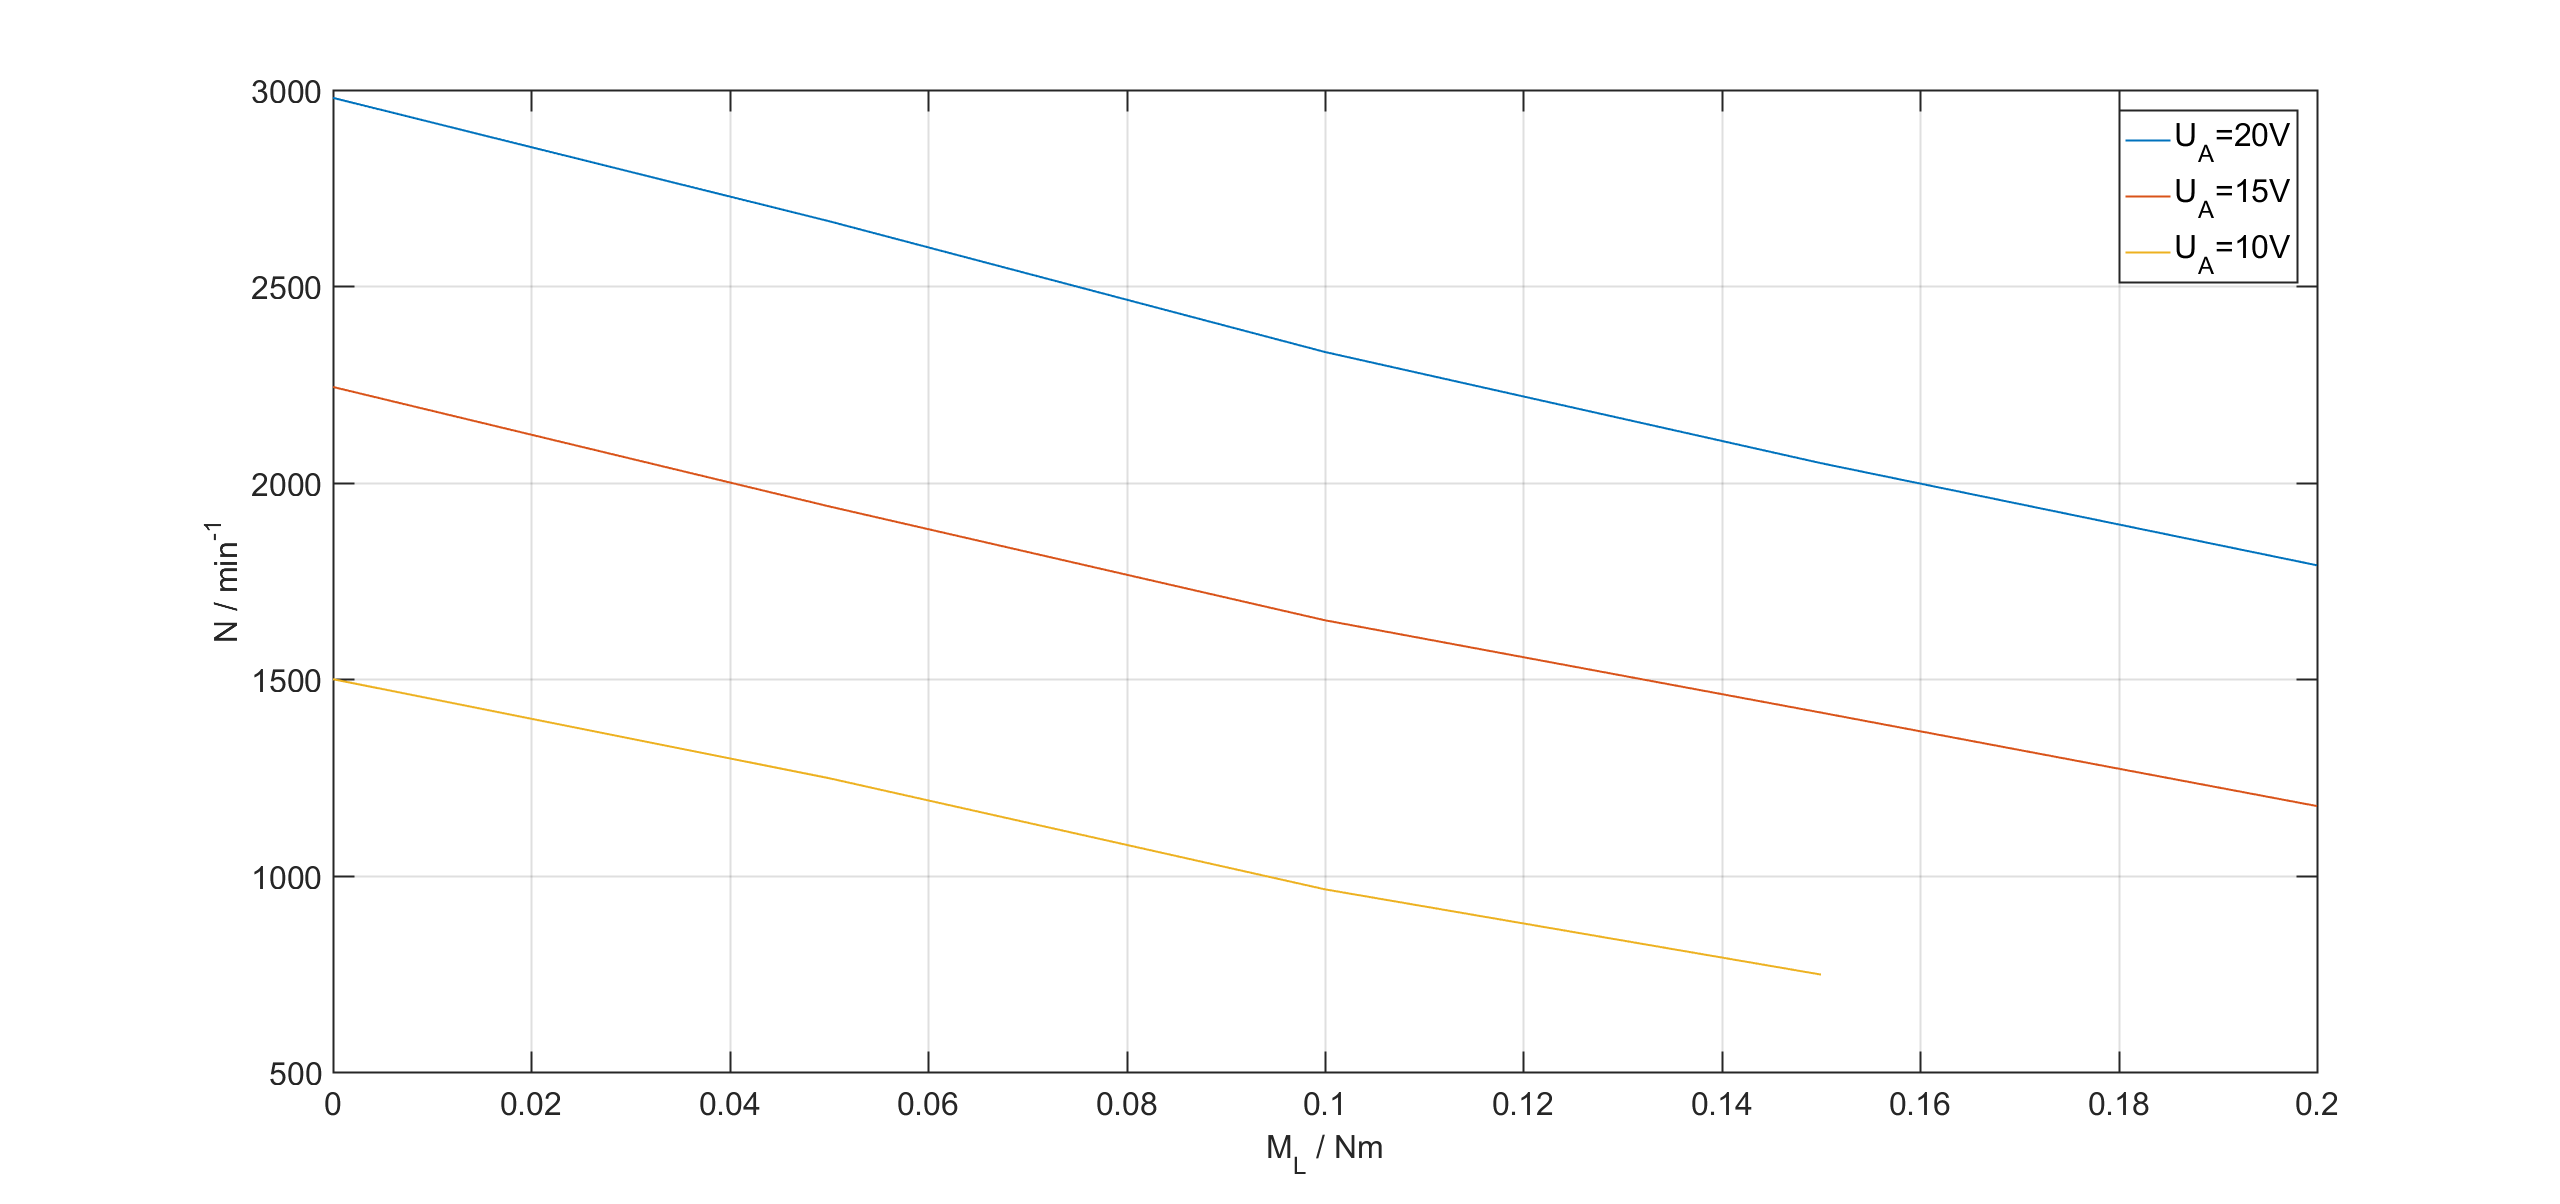
\includegraphics[width = \textwidth]{./Bilder/Drehzahldrehmomentkennlinie}
	\caption{Drehzahl-Drehmomentkennline}
	\label{fig:drehzahldrehm}
\end{figure}
%
\section{}\label{sec:aufg5b}
%
In Abb. \ref{fig:drehzahldrehm} erkennt man, dass es bei einer Ankerspannung von 10V nicht möglich ist, ein Drehmoment von 0.2Nm zu erreichen. Dies rührt daher, dass der BLDC einen DC-Motor antreibt, welcher generatorisch wirkt und somit eine Spannung erzeugt. Diese verursacht einen Stromfluss durch einen veränderlichen ohmschen Widerstand, dessen Größe durch den Laststrom-Regler angepasst werden kann. Bei 10V hat der BLDC eine bestimmte Drehzahl, somit kann nur eine bestimmte Spannung am Generator erzeugt werden. Der größtmögliche Strom am DC-Motor und damit auch das maximal erreichbare Lastmoment wird nach dem ohmschen Gesetz durch die Größe des Widerstands begrenzt. Selbst wenn dieser den kleinsten möglichen Wert annimmt, wird lediglich ein Strom von ca. 3A und das entsprechende Drehmoment von ungefähr 0,15Nm erzeugt.